
\section{Background}


%\subsection{Quantization}
%Quantization is another technique that is often used together with DSC to accelerate model execution of CNN models \FIXME{\cite{}}. When
%applying quantization to convolutions, the inputs and filter parameters are typically converted from 32-bit floating point (FP32) numbers
%to 8-bit integer (INT8) numbers. The convolution results will then be converted back to FP32. In this work, we focus on  post-training
%quantization \cite{fang2020post,jacob2018quantization} that converts the filters of a pre-trained CNN model to INT8 integers offline and
%the inputs to INT8 integers during runtime.





\subsection{GPU Architecture\label{sec:ga}}
Deep learning models are often trained and executed on the GPU. Modern GPUs employ a complex execution pipeline and memory hierarchy to
support concurrent execution of parallel threads. A typical GPU consists of multiple Streaming Multiprocessors (SMs). Each SM includes
multiple Single-Instruction-Multiple-Thread (SIMT) units, each of which has multiple lanes of execution. Threads scheduled in the same SIMT
unit are called a warp, which is the smallest scheduling unit in GPU. Like a modern CPU, a GPU consists of multiple memory hierarchies. The
thread-local registers are the fastest memory component, having the lowest access latency (1-2 cycles). The SM local L1 caches and shared
memory provide a larger storage capacity over the thread-local registers but have modestly higher accessing latency of around 30 cycles
\cite{mei2016dissecting,jia2018dissecting}. All the SMs share a unified L2 cache that provides an accessing latency of about 200 cycles.
The off-chip global memory, similar to the RAM in a CPU system, provides the largest memory storage capacity on the GPU but has the longest
accessing latency of around 500 cycles measured through running micro-benchmarks on NVIDIA RTX 2080Ti GPU used in this work. Local memory
resides in global memory and is used to hold variables with dynamic indexing or too large to fit into registers. It has the same access
latency as global memory. The key to optimizing memory performance is to make use of the fast memory sub-systems (i.e., registers and
shared memory) and reduce the number of memory accesses to slower memory. Our work is designed to provide such capabilities for depthwise
separable convolution operations.
\begin{figure}[t!]
\centering
  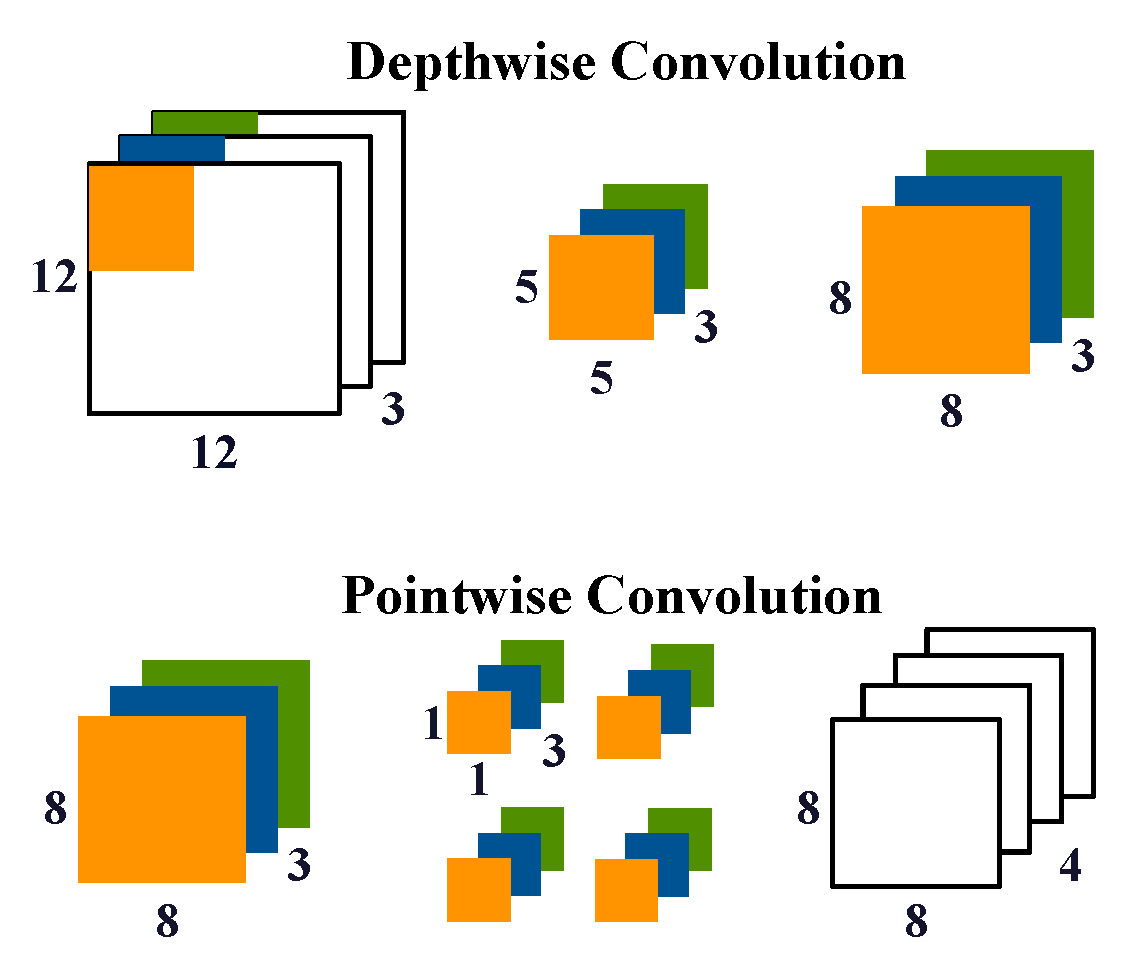
\includegraphics[height=5.5cm]{./figure/depthseparableconv.eps}
  \caption{Demonstration of depthwise convolution (above) and pointwise convolution (below).}
  \label{fig:depsepconv}
\end{figure}

\subsection{Depthwise Separable Convolution}
Our work targets depthwise separable convolution (DSC) that is widely used by  CNN  models to reduce the number of multiplication
operations needed for doing convolution (a standard operation in CNN). The DSC splits a standard depthwise (e.g., multi-channeled) 2D
convolution kernel into two individual kernels: a depthwise convolution kernel and a pointwise convolution kernel.

The depthwise
convolution kernel processes one input channel at a time, and stacks the outputs of all channels together to form an $n \times n \times c$
matrix, where $n \times n$ is the output of a depthwise convolution kernel and $c$ is the number of channels to be processed. Specifically,
it takes as input a feature map and applies a bank of 2D filters (e.g., an $N \times N$ kernel) on the width and height directions of
the input. We iteratively apply the depthwise convolution kernel to all channels. The above part of Fig. \ref{fig:depsepconv} shows an example of depthwise convolution, where three $5 \times 5$ 2D filters are used to convolve with the corresponding channel of a $12 \times 12 \times 3$ feature map and generate one $8 \times 8 \times 3$ output.

The output of the depthwise convolution kernel is fed
into a pointwise convolution kernel which uses a $1 \times 1$ filter to iterates through every single point. This kernel has a depth of the
number of input channels (i.e., $c$). The DSC reduces the computation by reducing the number of input transformations needed when compared
to a standard depthwise convolution. The below part of Fig. \ref{fig:depsepconv} shows an example of pointwise convolution, where four $1 \times 1 \times 3$ filters are used to convolve with the $8 \times 8 \times 3$ feature map iteratively and each filter generate one channel of a $8 \times \times 3$ output.


\subsection{Roadmap and Notations\label{sec:roadmap}} We present our approach for optimizing the two convolutional kernels of DSC in
Sections \ref {sec:strategies} and \ref {sec:pwconv}. We start by introducing our methods for improving data locality of depthwise
convolution in Section \ref{sec:strategies} and then presenting our approach for using dynamic work distribution to accelerate
small-batch-sized pointwise convolution in Section \ref {sec:pwconv}.

\mypara{Notations.} Throughout the paper, we use $I$, $F$, and $O$ to represent the input, the filter, and the output respectively; we also
use $N$, $C$, $H$, and $W$ to denote the batch size, the channel, the height, and the width, respectively.
